
\chapter{Projekt i implementacja algorytmu generującego plan lekcji}

\section{Wstęp}
Problem ułożenia najlepszego planu zajęć jest problemem Np-Zupełnym. W projekcie zostało zaimplementowane podejście ewolucyjne. Na rysunek ~rysunku~\ref{rys:time_table_dia} została zobrazowana struktura generowanego planu zajęć.

\begin{figure}[h]
\centering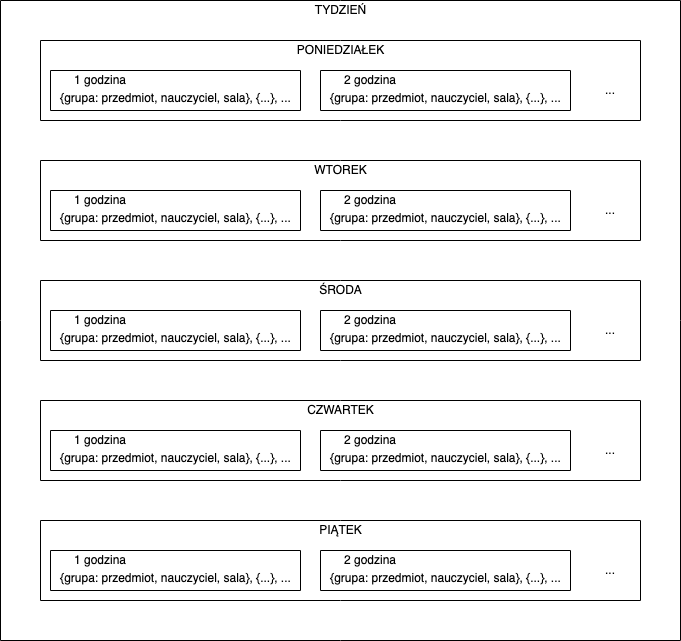
\includegraphics[width=\textwidth]{figures/time_table_dia}
\caption{Struktura planu zajęć}\label{rys:time_table_dia}
\end{figure}


Zagadnienie implementacji algorytmu można podzielić na cztery główne części: 
\begin{itemize}
	\item przygotowanie danych wejściowych,
	\item ułożenie planu zajęć,
	\item ocena planu zajęć,
	\item ewolucja planu zajęć.
\end{itemize}


\section{Przygotowanie danych wejściowych}
    
    Przygotowanie danych wejściowych jest kluczowe w działaniu algorytmu. Na podstawie danych otrzymanych od back-end, zostaje ułożona lista czteroelementowych krotek, gdzie pierwszym elementem jest nazwa grupy, drugim elementem jest nazwa przedmiotu, trzecim elementem jest nazwa nauczyciela, a czwartym elementem jest nazwa sali. Wartość elementu sali jest na początku wartością pustą null, a wartość elementu nauczyciela, jest wartością pustą null, wtedy i tylko wtedy kiedy nie został wskazany nauczyciel dla konkretnej klasy. W takiej liście znajdują się wszystkie jednostki lekcyjne występujące w całej szkole. Przykładowo jeżeli pewna klasa IIC ma mieć 5 matematyk w tygodniu z nauczycielem Jan Kowalski, to do listy dostanie dodane pięć krotek postaci (IIC, matematyka, Jan Kowalski, null). Struktura wspomnianej listy znajduje się na ~rysunku~\ref{rys:krotki}.


\begin{figure}[]
\begin{tabular}{llll}
NAZWA GRUPY & NAZWA PRZEDMIOTU & NAZWA NAUCZYCIELA & NAZWA SALI \\
IIC         & matematyka       & Jan Kowalski      & null       \\
IIC         & matematyka       & Jan Kowalski      & null       \\
IIC         & matematyka       & Jan Kowalski      & null       \\
IIC         & język polski     & Andrzej Nowak     & null       \\
IIC         & język polski     & Andrzej Nowak     & null       \\
IA          & język polski     & null              & null      
\end{tabular}
\caption{Struktura listy krotek} \label{rys:krotki}
\end{figure}

\section{Ułożenie poprawnych planów zajęć}

    Głównym założeniem układania planu zajęć jest to, że na podstawie tej samej listy krotek, zawsze zostanie wygenerowany konkretny plan zajęć. 
Układanie planu zajęć przebiega następująco:
\begin{enumerate}
	\item z listy krotek zostaje zabrana pierwsza z brzegu krotka,
	\item wybrana krotka zostaje przydzielona do pierwszej możliwej konkretnej godziny w 		\item konkretnym dniu (czyli do takiej jednostki godzinowej, wtórej są spełnione 			\item wprowadzone przez użytkownika założenia oraz jest wolna sala),
	\item poprzednie czynności zostają powtarzane tak długo, aż cała lista zostanie przeiterowana.
\end{enumerate}
Jeżeli po zakończeniu działania procesu układania planu zajęć lista krotek nie będzie pusta, to ułożony plan zajęć jest niekompletny i niepoprawny. Proces układania planu zajęć został przedstawiony na ~rysunku~\ref{rys:time_table_prep}.

\begin{figure}[h]
\centering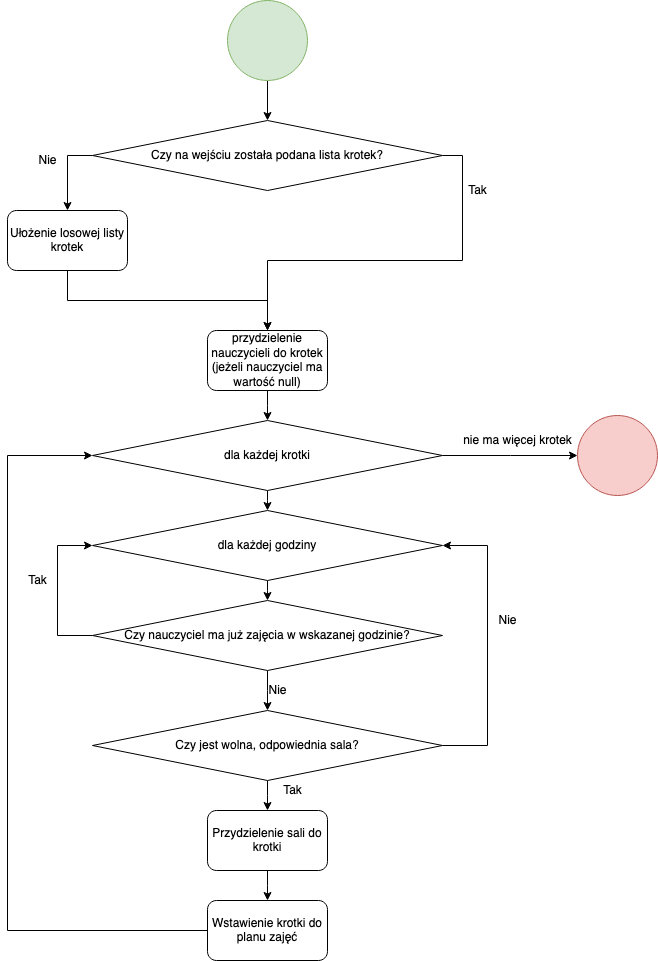
\includegraphics[width=\textwidth]{figures/time_table_prep}
\caption{Proces układania planu zajęć}\label{rys:time_table_prep}
\end{figure}

\section{Funkcja oceny}

    Funkcja oceny przyznaje planu zajęć pewną ilość punktów. Ocena może mieć wartość z zakresu od minus nieskończoności do 0, gdzie im wartość większa, tym lepsza ocena.
    Wpływ na końcową ocenę mają następujące elementy:
\begin{enumerate}
	\item liczba tzw. okienek występujących w planie zajęć każdego nauczyciela,
	\item liczba tzw. okienek występujących w planie zajęć każdej grupy,
	\item liczba trudnych przedmiotów w ciągu jednego dnia w planie zajęć każdej grupy,
	\item liczba sytuacji, w których grupa ma rozdzielone zajęcia tego samego przedmiotu innym przedmiotem (np. 1 godzina lekcyjna - matematyka, 2 godzina lekcyjna - biologia, 3 godzina lekcyjna - matematyka),
	\item liczba sytuacji, w których zajęcia wychowania fizycznego nie występują na początku lub na końcu planu zajęć dnia.
\end{enumerate}


\section{Ewolucja planów zajęć}

    Część ewolucyjna algorytmu wykorzystuje wszystkie poprzednie części. Na początku algorytm generuje pewną populację planów zajęć, która będzie nazywana dalej pierwszą generacją. Zawartość listy krotek jest identyczna dla każdej jednostki z populacji, ale kolejność krotek w liście jest pseudo losowo zmieniona. Dzięki takiemu rozwiązaniu, każda jednostka w populacji może wygenerować zupełnie inny plan zajęć. Za pomocą funkcji oceny, do każdego z planów zostaje przydzielona pewna ilość punktów. 

Połowa najgorzej ocenionych planów zostaje zabita. Z każdego planu zajęć, któremu udało się przeżyć, generowany jest kolejny plan. Plan, z którego został wygenerowany nowy plan, będzie nazywany w dalszej części pracy rodzicem, natomiast nowo wygenerowany plan będzie nazywany potomkiem. Lista krotek potomka, będzie zawierała tą samą kolejność co rodzic, ale losowo wybrane rekordy zamienią się w sposób pseudolosowy pozycjami w liście, taka zamiana będzie nazywana dalej mutacją. Nowo wygenerowane jednostki zostają ocenione oraz dodane do populacji, w ten sposób powstaje druga generacja planów zajęć.

    Czynność z poprzedniego akapitu powtarza się jeszcze g-razy, gdzie g to liczba wszystkich generacji. Działanie całego algorytmu zostało przedstawione na ~rysunku~\ref{rys:alf_flow}.


\begin{figure}[h]
\centering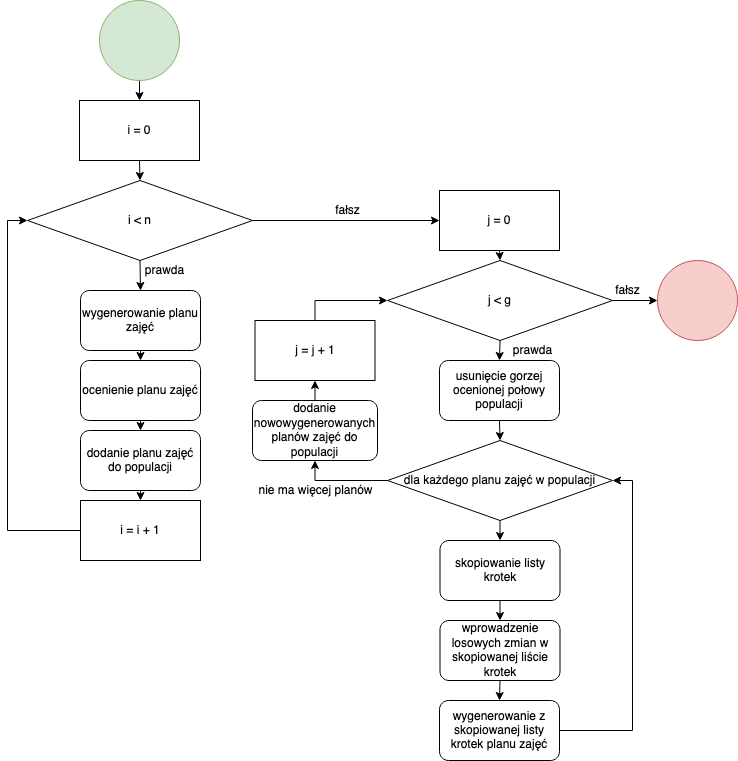
\includegraphics[width=\textwidth]{figures/alg_flow}
\caption{Algorytm - diagram}\label{rys:alf_flow}
\end{figure}



